\section{Query Construction Algorithm}

\begin{figure*}
\centering
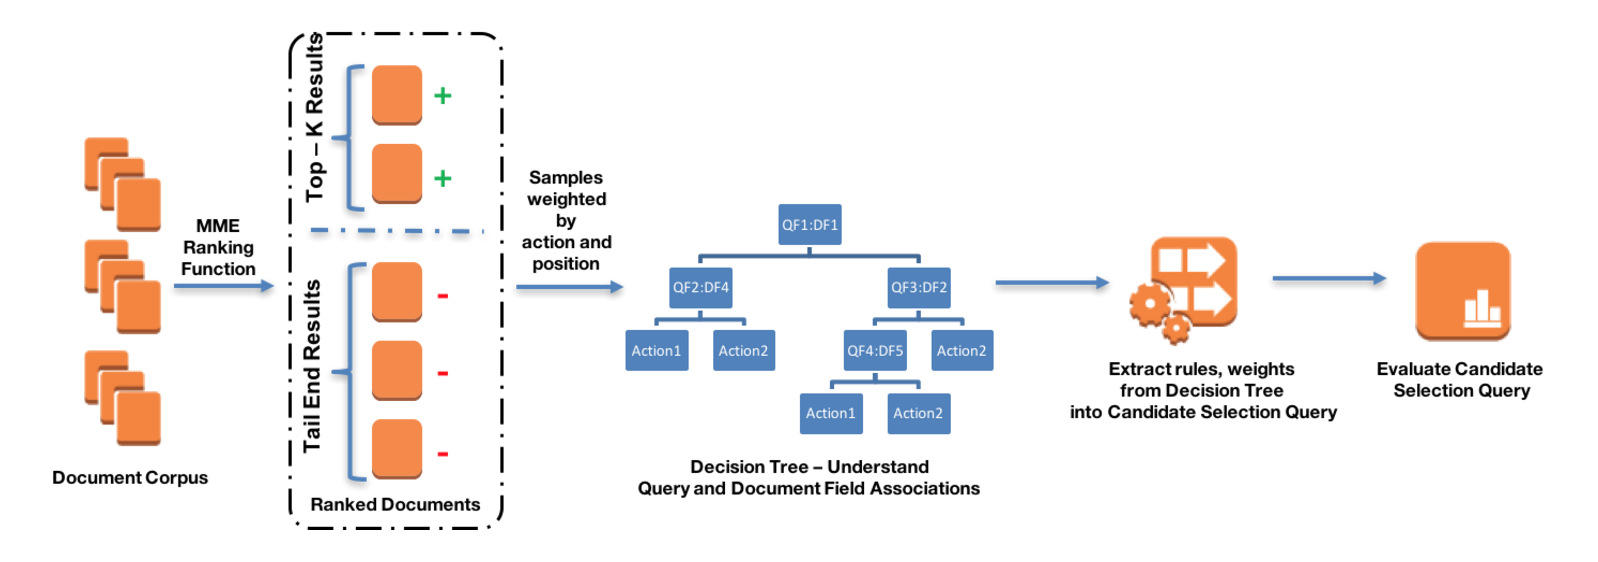
\includegraphics[width=\textwidth]{training-process.png}
\caption{Offline Training Process}
\label{fig:offline-training-process}
\end{figure*}


In this section, we describe the core algorithm used for query construction.
The entire flow is depicted in Figure~\ref{fig:offline-training-process} and
detailed below.
The algorithm consists of two steps:
\begin{enumerate}
    \item Construct decision tree using offline replay data
    \item Convert the decision tree into query clauses with weights. These
    weights will then be used in the WAND operators described in Section~[\ref{sec:wand}].
\end{enumerate}

The process of constructing decision trees and extracting clauses can be iterative. The depth of the decision tree is a hyper
parameter which can be tuned based on the output of the clauses. We will
describe details in this section.

\subsection{Decision Tree Construction}

The decision tree construction which in turn can be used for query
construction is described in Algorithm~\ref{alg:decision-tree2}. The branching
variables in the decision trees are all features described below. Consider $J_f$ 
and $M_f$ to be relevant fields in job details
and member profiles respectively. All {\it cross matches} in $J_f \times M_f$ are
potentially cross features which can be used as query clauses as well as
branching points in decision trees. Example, consider field in the job called
{\it Job Title} and a member profile field called {\bf Member Current Title}, a
potential feature would be {\it Job Title matches member current title}. Other
similar examples include:
\begin{enumerate}
    \item Job location matches member profile location
    \item Job company size matches member preference for company size
\end{enumerate}
Let $F$ represent the cumulative set of such features. We first sample set of
queries from production (say $Q$). We then run each query in this set through
our offline replay framework. Offline replay ranks the document set as well as
extracts the value of features in the feature set $F$. Assuming that the
original ranking is not bad (a reasonable assumption), we could use the top
$k_1$ results as positive and bottom $k_2$ as negative. We then have a dataset
of features and labels which can be run through pretty much any decision tree
based algorithm~\cite{quinlan1986induction} to extract a tree. 


\begin{algorithm}
\caption{Decision Tree Construction}\label{alg:decision-tree2}
\begin{algorithmic}[1]
  \State \textbf{Input}: User and query logs with queries, member activity, member profile and job
  details.
  \State \textbf{Output}: Decision tree Graph $G(V, E)$.
  $v \in V$ represents a feature, edge $e \in E$ to be represented by the tuple
  $(u, v, d, w)$ where $(u, v)$ represent nodes, $d$ represents the decision
  and $w$ represents the weight.
  \State Derive feature set $F$ which consists of cross query level cross
  features between job details and member profiles
  \State Sample queries from production into query set $Q$
  \State $T \gets \emptyset$
  \For {query $q \in Q$}
    \State Generate top $K$ results
    \State Extract features for each result
    \State Mark top $k_1$ results as positives $P$
    \State Mark bottom $k_2$ results as negatives $N$
    \State $T \gets T \cup P \cup N$
  \EndFor
  \State Run any standard decision tree algorithm on training set $T$ to get
  decision tree graph $G(V, E)$. 
  \State Use entropy at the decision tree edges to derive weight of each edge.
  \State %newline
\end{algorithmic}
\end{algorithm}

\subsection{Query Construction}

The entire to construct the queries is shown in
Algorithm~\ref{alg:query-construction}. The input to the algorithm is query
logs and some hyper parameters. These hyper parameters control the depth of the
tree as well as the number of positive and negative labels needed to get an
appropriate query clause. Like any decision tree, we expect to know the number
of positive and negative labels at each leaf node. The algorithm goes through a
loop terminating when a suitable solution is found or maximum tree depth is
reached. We start with min depth and construct a decision tree. Once the tree
is constructed, we enumerate all paths and cut off at a point when the number of
positive samples (at leaf nodes of each path) is more than a certain fraction
of the total positives. We also need to make sure that the number of negative
samples is low enough. If the constraint for both positive and negative samples
is met, we stop and return the path. If not, we try to build a deeper tree.

To give a general idea of how the queries are constructed we can look at a sample decision tree in Figure ~\ref{fig:decision-tree}.
Let us assume total positive coverage $\alpha$ is $0.06$ and hyper parameter $\beta$ is $0.04$. We describe the query construction in the following steps: 

\begin{enumerate}
    \item Let's say we have a member $M$ with following fields:
    \begin{itemize}
    \item Current Title = Software Engineer
    \item Member Seniority = Entry Level
    \item Member skill = Computer Science
    \end{itemize}
    \item We use standard depth first search on our decision tree to extract all the paths starting from root to leaf. We will refer to this set as $S_c$.
    \item $S_c$ is then sorted by number of positives labels that each path holds. We define the number of positives in a set by $P_+$ and number of negatives by $P_-$
    \item We iterate over the set $S_c$ to find a subset $S_c'$ which satisfy the constraint that $P_+'$ is greater $\alpha * P_+$ and $\frac{numNegativeLabels(P_{-})}{numPositiveLabels(P_{+})} \leq \beta$. 
    \item In our example, the paths indicated in green color satisfies the above constraints, since $P_+'= 5000$  is greater than $P_+ * \alpha = 4320$ and  $P'_-/P'_+ = 0.03 \leq \beta$
    \item All the paths in subset $S_c'$ can then be constructed as a OR Lucene query~\cite{mccandless2010lucene} where each path is an AND of features. In our example we have total four paths starting from root to leaf and only two paths marked in green color satisfy the constraints. Constructed query $CQ$ formed  using set of all valid paths $S_c'$ and  a member $M$ will look like the following: 
    \begin{itemize}
    \item \lucenequery{+(?(+jobTitle:Software Engineer +jobSkill: Computer Science) ?(+jobTitle:Software Engineer -jobSkill:Computer Science))}
    \end{itemize}
    \item The entropy measure at each node can be used directly to get the
        weights if we need to use a WAND query
    
\end{enumerate}

\begin{algorithm}
\caption{Query Construction}\label{alg:query-construction}
\begin{algorithmic}[1]

    \State \textbf{Input}: Query logs $Q_l$ with member activities, job details
    and member profile. $\alpha$ hyper parameters representing
    percentage of positives we want to cover. $\beta$ hyper parameter
    representing the min ratio of positives to negatives. $h_{max}$ and $h_{min}$ represent
    the maximum and minimum depth of the decision tree respectively.
    \State \textbf{Output}: Query clauses for search or recommendations
    \Function{constructClauses}{$\alpha$, $\beta$, $h_{max}$} 
        \State $h$ $\gets$ $h_{min}$
        \While {True}
            \State $G(V,E) \gets \Call{decisionTreeLearner}{Q_l, h}$
            \State $P \gets allPaths(G)$
            \State Sort $P$ by numPositiveLabels
            \State $P_{+} \subseteq P$ such that numPositiveLabels($P_+$) $\geq \alpha * numPositiveLabels(P)$
            \State 
            %\If{$\frac{numPositiveLabels(P_+)}{numNegativeLabels(P_{_})} \geq \beta$ or $h \geq h_{max}$}
            \If{$h \geq h_{max}$ or $\frac{numNegativeLabels(P_{-})}{numPositiveLabels(P_{+})} \leq \beta$}
                \State break     
            \EndIf
            $h \gets h + 1$
            \State 
        \EndWhile
        Clauses = extractClauses($P_+$)

    \EndFunction

\end{algorithmic}
\end{algorithm}



\begin{figure*}
\centering
    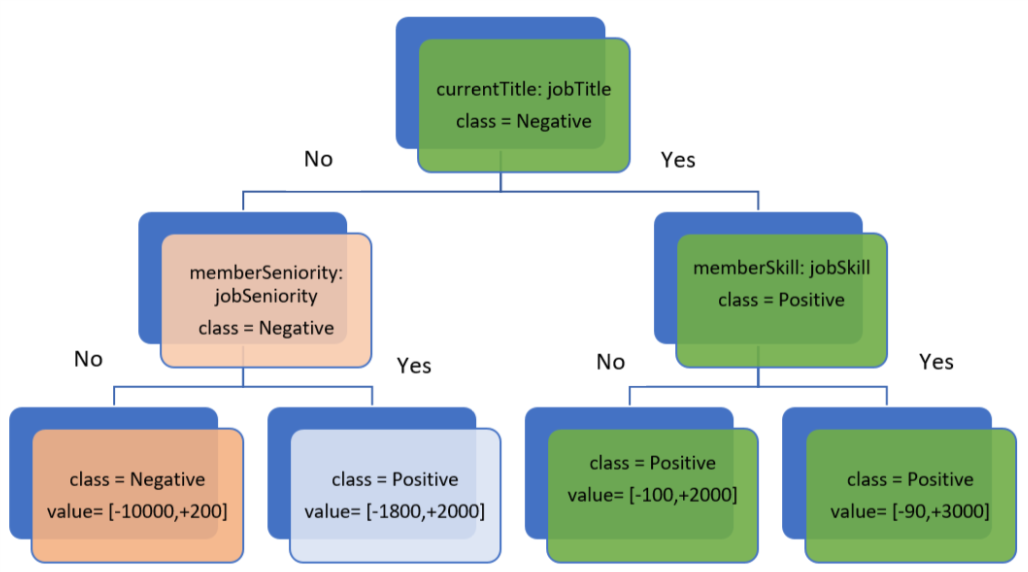
\includegraphics[width=\textwidth]{decision-tree-final.png}
\caption{Decision Tree}
\label{fig:decision-tree}
\end{figure*}
